% Using KOMA Script document style
% Font size setting and
% option to skip empty lines as new paragraphs
\documentclass[10pt,a4paper]{article}
% Packages without Options
\usepackage{
	algorithm,
	alltt,
	algpseudocode,
	amsfonts,
	amssymb,
	appendix,
	array,
	booktabs,
	dirtree,
	enumitem,
	float,
	footnote,
	gensymb,
	geometry,
	graphicx,
	interval,
	karnaugh-map,
	lipsum,
	listings,
	longtable,
	makecell,
	mathtools,
	minted,
  nicematrix,
	parskip,
	pdfpages,
	pgfkeys,
	pgfplots,
	subcaption,
	tabularx,
	tablefootnote,
	textcomp,
	tikz,
    titlecaps,
	venndiagram,
	wrapfig,
	wrapfig,
	xcolor
}



% Packages with Options

\usepackage[framemethod=tikz]{mdframed}
\usepackage[colorlinks,linkcolor=cyan, citecolor=cyan, urlcolor=cyan]{hyperref}
\usepackage[labelfont=bf,textfont=it,labelsep=period]{caption}
\usepackage[RPvoltages]{circuitikz}
\usepackage[english]{babel}
\usepackage[nameinlink,noabbrev]{cleveref}

\definecolor{mintedbackground}{rgb}{0.97,0.97,0.97}

\setminted[cpp]{
bgcolor=mintedbackground,
    linenos=true,
    breaklines=true,}

\setminted[js]{
bgcolor=mintedbackground,
    linenos=true,
    breaklines=true,}

\setminted[python]{
bgcolor=mintedbackground,
    linenos=true,
    breaklines=true,}
    

\linespread{1.5}

% Package: AlgorithmicX
% Sets all comments to be indentend and aligned

\renewcommand{\Comment}[2][.7\linewidth]{%
  \leavevmode\hfill\makebox[#1][l]{//~#2}}


% Package: Interval
% Sets the style of mathematical intervals
\intervalconfig{
soft open fences, separator symbol=,,
}

% Package: Geometry
% Sets the page margins
\geometry{
    a4paper,
    left=32mm,
    right=22mm,
    top=22mm,
    }
	
% Creates a proper caption name for algorithms
\newcommand{\algorithmautorefname}{Algorithm}
\newcommand{\listingautorefname}{Listing}
\algrenewcommand{\algorithmiccomment}[1]{\texttt{// #1} }
% Creates a numbered environment for Theorems
\newtheorem{theorem}{Theorem}

% Redefine the implication arrow to be a simple, thin arrow instead of the default, thick arrow
\renewcommand{\implies}{\rightarrow}

% Create a new command for the set complement to make my logical statements easier to read
\newcommand{\compl}{\overline}

% Creates commands for combinatorics nCr and nPr
\newcommand{\nCr}[2]{\,_{#1}C_{#2}} % nCr
\newcommand{\nPr}[2]{\,_{#1}P_{#2}} % nPr

% Package: tikz
% Loads libraries for drawing automata, 
\usetikzlibrary{automata,positioning,shadows,arrows, shapes.gates.logic.US, calc}

% Creates a command to create a button shape
\newcommand*\keystroke[1]{%
  \tikz[baseline= (key.base)]
    \node[%
      draw,
      fill=white,
      drop shadow={shadow xshift=0.25ex,shadow yshift=-0.25ex,fill=black,opacity=0.75},
      rectangle,
      rounded corners=2pt,
      inner sep=1pt,
      line width=0.5pt,
      font=\scriptsize\sffamily
    ] (key) {#1\strut};
}

% Package: pgfplot
% Sets the global options for PGF Plots
\pgfplotsset{compat=newest}

% Package: tikz
% Flowchart Shapes
\tikzstyle{startstop} = [rectangle, rounded corners, minimum width=3cm, minimum height=1cm,text centered, draw=black, fill=red!30]
\tikzstyle{io} = [trapezium, trapezium left angle=70, trapezium right angle=110, minimum width=3cm, minimum height=1cm, text centered, draw=black, fill=blue!30]
\tikzstyle{process} = [rectangle, minimum width=3cm, minimum height=1cm, text centered, draw=black, fill=orange!30]
\tikzstyle{decision} = [diamond, minimum width=3cm, minimum height=1cm, text centered, draw=black, fill=green!30]
\tikzstyle{arrow} = [thick,->,>=stealth]

% Disable Minted syntax error highlights (red boxes)
\AtBeginEnvironment{minted}{%
  \renewcommand{\fcolorbox}[4][]{#4}}

% Listings Style (non-minted)

\lstdefinestyle{arjuncode}{
    basicstyle=\ttfamily,
    breakatwhitespace=false,         
    breaklines=true,                 
    captionpos=b,                    
    keepspaces=true,                 
    numbers=left,                    
    numbersep=5pt,                  
    showspaces=false,                
    showstringspaces=false,
    showtabs=false,                  
    tabsize=2
}

\lstset{style=arjuncode}

\graphicspath{{images/}}

 %Adjust this based on where your Summary is stored
\title{CM3010: Databases and Advanced Data Techniques \\ Midterm Assignment}
\author{Arjun Muralidharan}
\begin{document}

\maketitle
\newpage
\tableofcontents
\listoffigures
\listoftables
% \listofalgorithms

\newpage
\renewcommand{\subsubsectionautorefname}{section\negthinspace}

\section{Find and critique a dataset}

\subsection{Finding the dataset}

I will use a dataset of sports matches, specifically test cricket matches from 2004 until 2021, obtained from \cite{rushe_2021}.

The data describes ball-by-ball statistics and can be considered \textbf{pre-existing external data}. It is assembled with automated \textbf{data curation} to assemble the data from various sources. Some general points on the structure of the data:

\begin{itemize}
    \item Each match's data is organised in a separate JSON file.
    \item Each file includes some meta data about the creation and the event that this match was part of.
    \item All ball-by-ball data is stored in \textbf{nested objects} within the JSON structure.
    \item This leads to lots of repetition of information as this follows a \textbf{tree-like} structure rather than a relational one.
\end{itemize}

Hence the data needs to be normalized and mapped to a relational model in order to use it in a relational database.

\subsection{Critiquing the dataset}

One advantage of the dataset is that it is very \textbf{up to date} as new matches are added every day. This makes the data set highly usable and accurate, at least starting from 2004 onwards. The dataset is also \textbf{lightweight to use} given that each match has it's own file; new data does not change or affect the size and integrity of previous data.

However, the data is distributed and hence \textbf{harder to consolidate} into a single repository, and it contains lots of repeated data as player names occur again for each individual delivery (a ball played) where the player was involved. Matches that belong to the same event or test match series are in separate files and the event name is repeated in all the files related to an event.

Event names are further not unique, e.g. "New Zealand tour of India" may have happened many times in the past 17 years, so the year of the event needs to be considered when defining what a unique event is.

\subsection{Interest in the data set}

I chose this data set as I personally enjoy watching Cricket as a sport, and believe the data set to be interesting for the following reasons:

\begin{itemize}
    \item Cricket is a statistics-heady sport, with lots of data recorded officially on a ball-by-ball basis
    \item Generally, sports data is rarely available in an openly available format and often hidden behind paywalls or graphical interfaces, gatekept by sports companies and sports news sites. This dataset made openly available a lot of information about this fascinating sport.
    \item The data is structured in an intersting manner that in its current form is not suited for relational representation and many questions cannot be answered without transforming the data into a relational form.
\end{itemize}

\subsection{Questions to answer}

By transferring a part of the data into relational form, I aim to answer the following questions which cannot be answered with the current source structure.

\begin{enumerate}
    \item How many test matches have the test-playing nations played since 2004?
    \item Who are the 10 batsmen with the highest number of runs scored since 2004?
    \item Which 10 players are the most successful bowlers in terms of wickets taken and runs conceded since 2004?
    \item What is the most common type of dismissal since 2004?
\end{enumerate}

\subsection{Model your data}

I have built a tentative ER diagram shown in \autoref{fig:er}. Some notes on normalization:

\begin{enumerate}
    \item The core entities are \textit{players} and \textit{matches}. A match in cricket is played through \textit{deliveries}, or individuall balls. Hence, players are involved in deliveries, and called up to line-ups to play in matches. These relationships are modelled with linking entities that would eventually result in link tables.
    \item This ER diagram is not a complete representation, as further, more granular normalization might be warrented based on the use case. For example, the entitiy \textbf{delivery role} might need an entity that stores the possible roles, from which an attribute is drawn (e.g. bowler, batter, fielder, etc.).
\end{enumerate}

\begin{figure}[H]
    \centering
    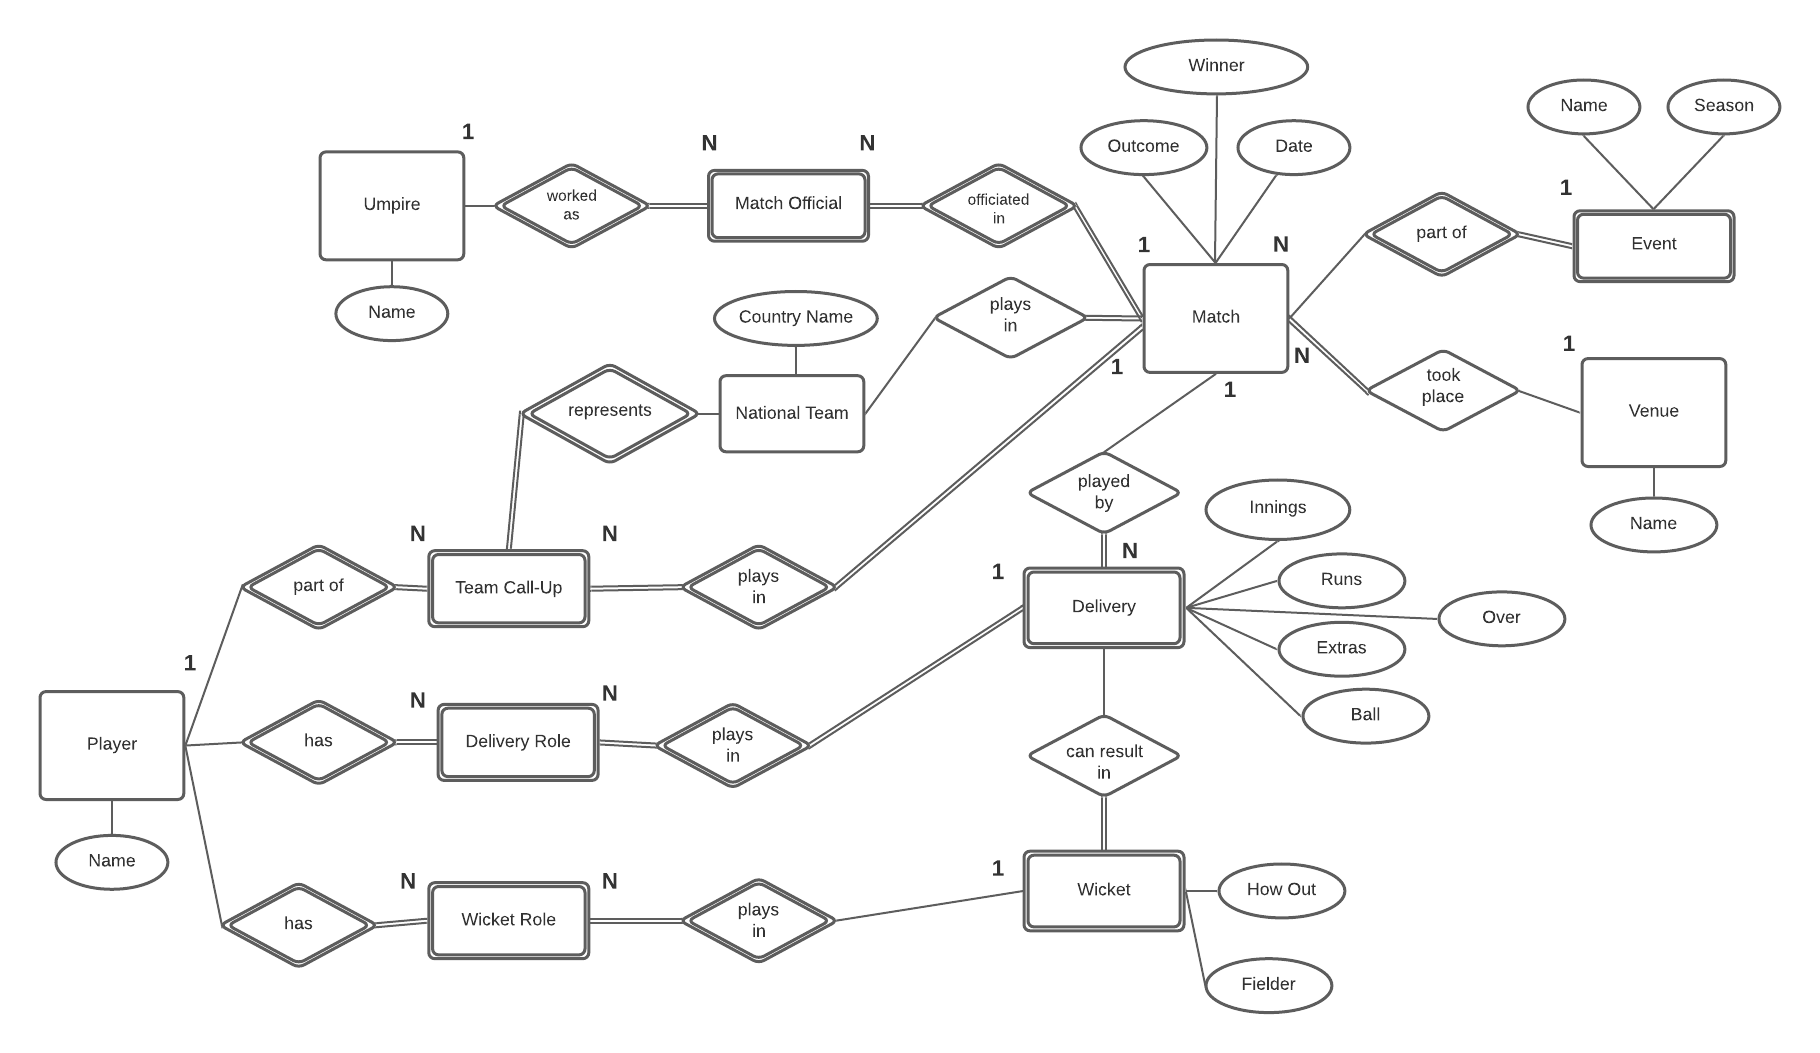
\includegraphics[width=\textwidth]{Cricsheet.png}
    \caption{ER diagram for Cricsheet data}
    \label{fig:er}
\end{figure}

\subsection{Create the database}

The database implementation does not completely reflect the ER diagram exactly, because the scope far exceeds the current needs of answering the questions. Therefore, I took a slightly simplified approach and did not implement every link table shown above. I recognize this shortcoming but want to demonstrate that implementing additional link tables would be trivial.

\begin{listing}[H]
    \tiny
    \caption{Listing: Database Implementation}
    \label{lis:db}
    \lstinputlisting{cricapp/db_setup.sql}
\end{listing}

Reflecting on this implementation, for a more scalable version I would implement more linking tables. Also, I have not implemented tables unneeded for the questions posed, such as Umpires, Events or Venues. If I were building a more full-fledged cricket scoring app, I would implement this analogously.

\subsection{Create a simple web application}

The web application is hosted in the lab environment. Some notes in running it:

\begin{enumerate}
    \item It can be started with the \texttt{npm start} command.
    \item The database is already populated, but can be re-populated by running \texttt{node db/cric.js}. This instantiates a class that processes the JSON files in the \texttt{matches} folder and adds them to the database. Because this operation can be long and heavy on the database, I decided to decouple this from running the application.
    \item The application requires about a minute (in the lab environemnt) to query the database, as I have not implemented any caching of query results. Because some queries need to sift through every ball every played since 2004, this takes a moment. The app presents a warning and asks you to refresh the page after waiting a minute.
\end{enumerate}

The app displays all the associated SQL queries on-demand. This functionality may not work in the lab environment as the browser preview can be slow and tedious to interact with; hence I recommend installing the app locally if desired.

\begin{figure}[H]
    \centering
    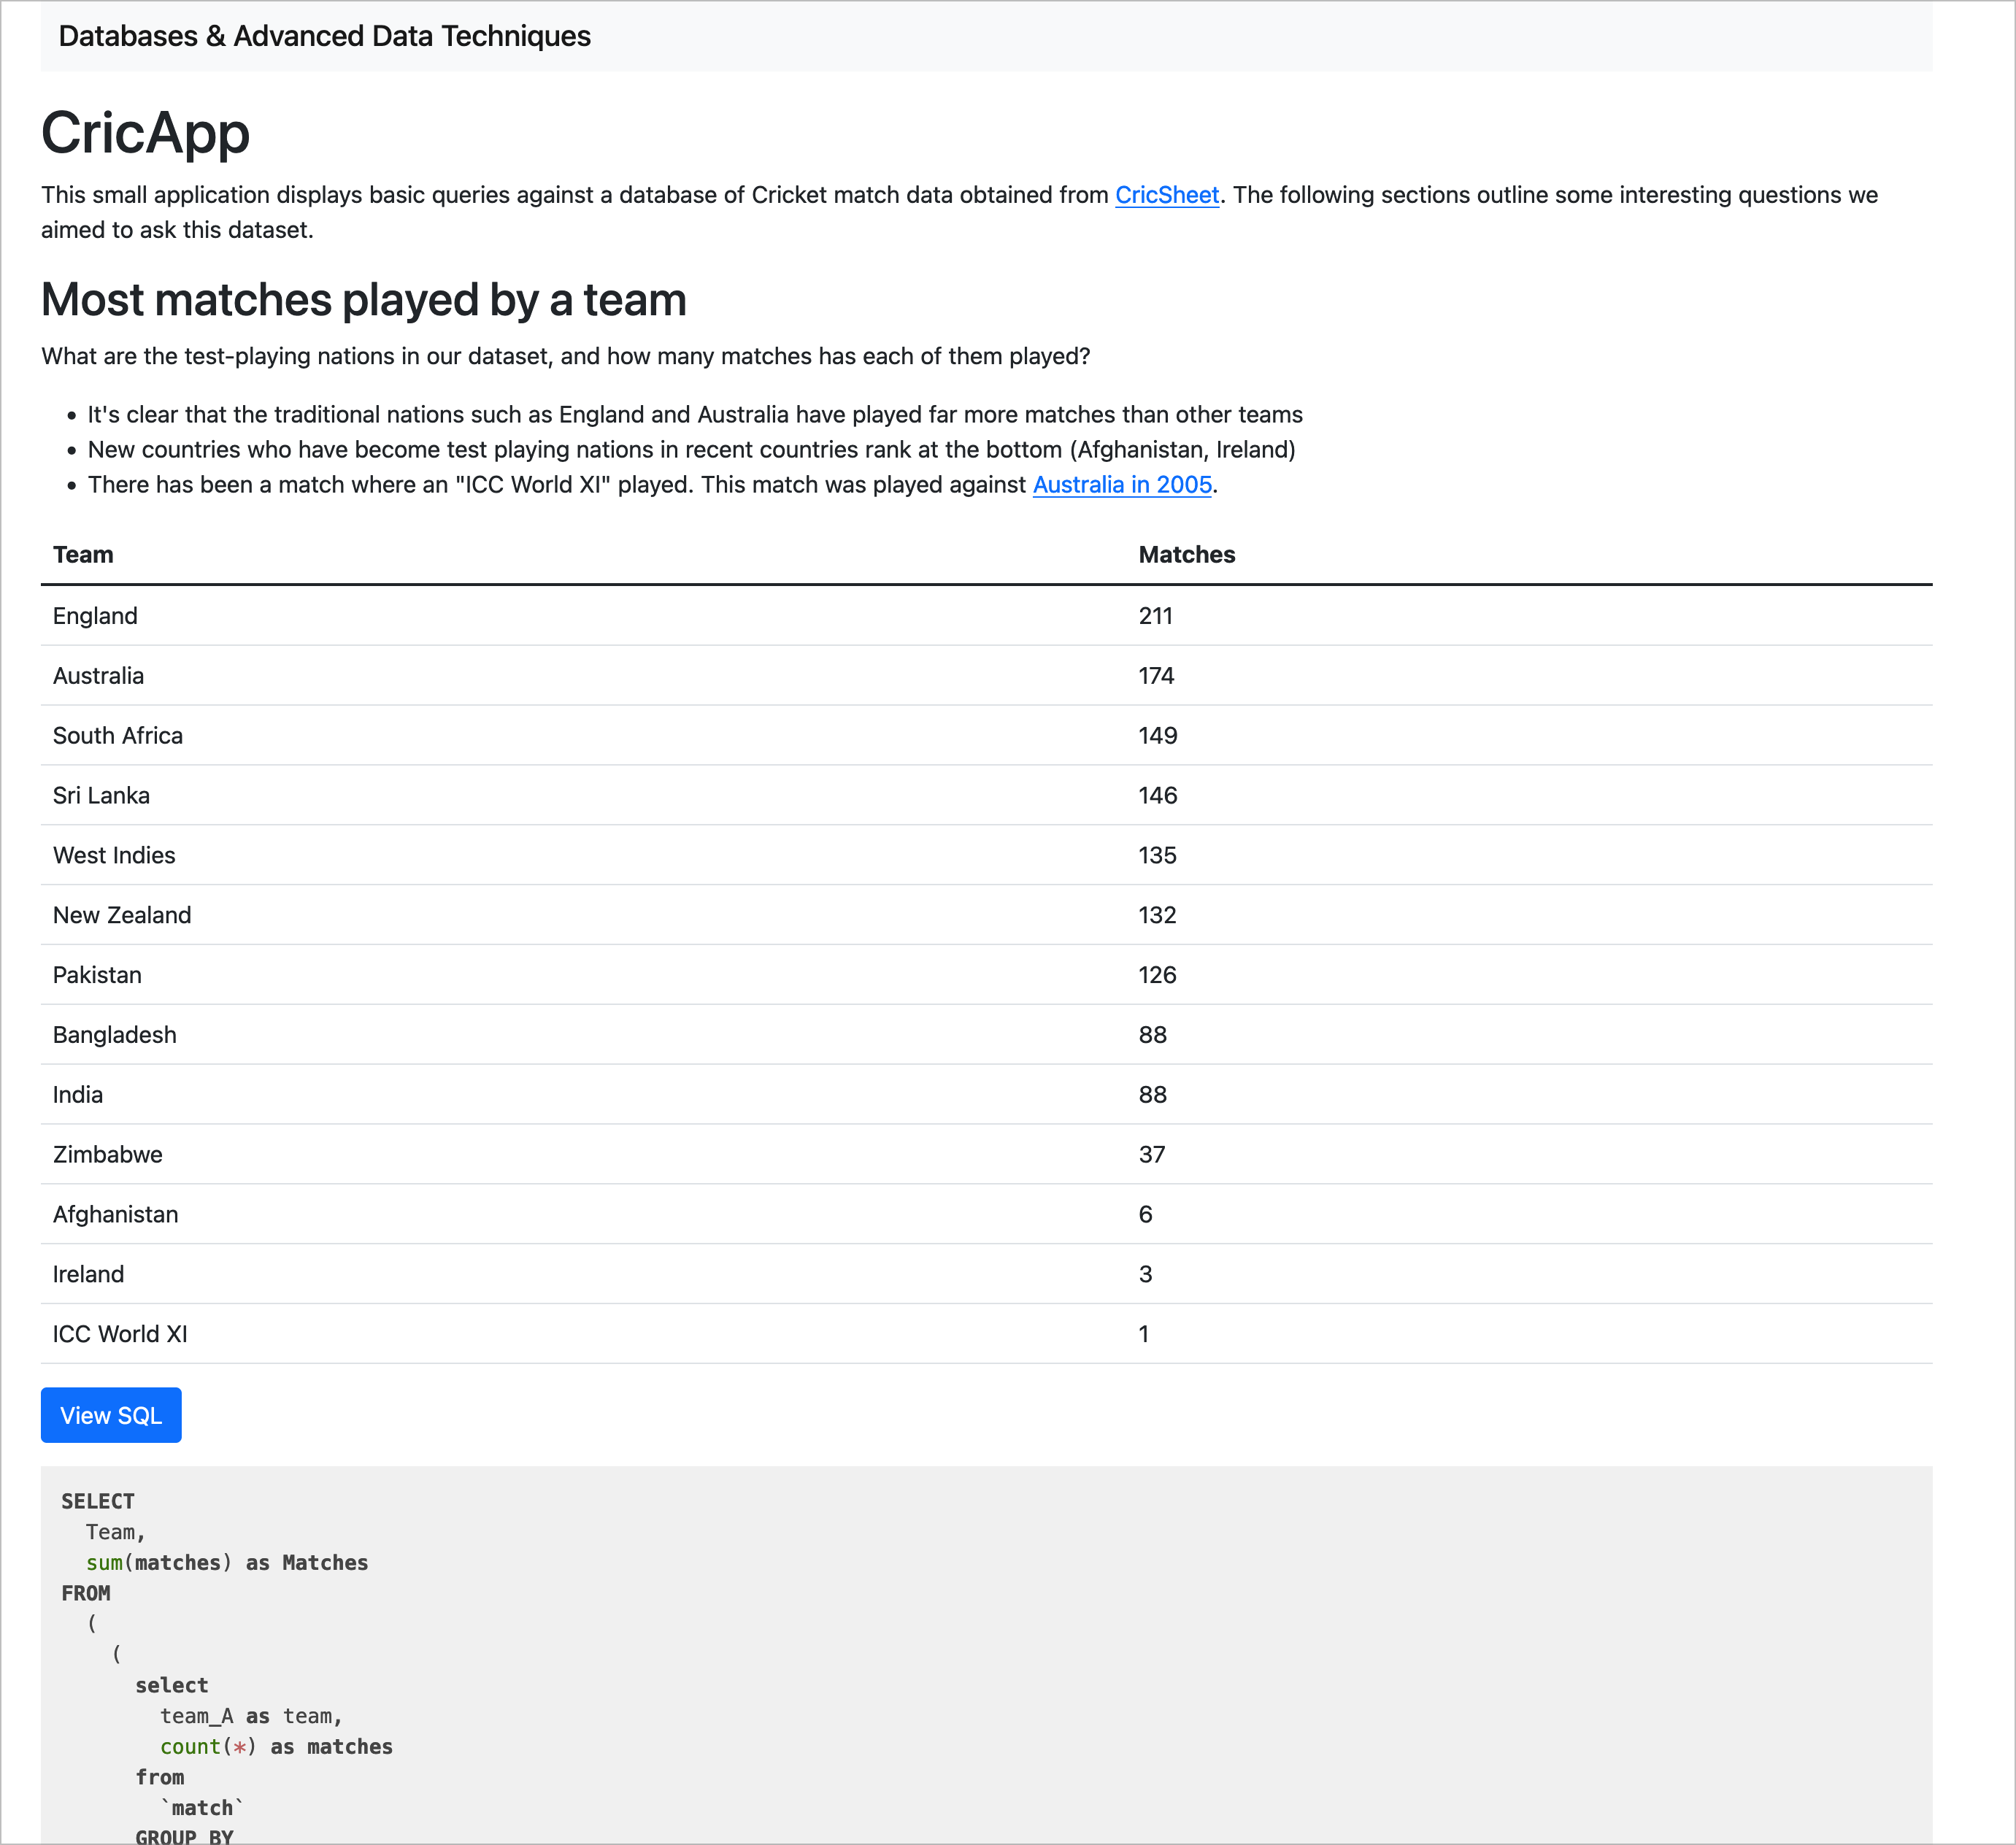
\includegraphics[width=\textwidth]{appshot}
    \caption{Screenshot of the working app}
    \label{fig:appshot}
\end{figure}

\bibliographystyle{IEEEtran}
\bibliography{bib}


\end{document}